\documentclass[../main]{subfiles}

\graphicspath{{../figures/}}

\begin{document}

\section{異常音の位置推定}
\label{sec:pmethod_abnormal_detection}
ここまで,学習済みモデルを利用してメルスペクトログラムから異常音のエネルギーを推定する手法について述べた.
本章ではこの異常音のエネルギーと自己位置のペアを利用して,異常音の位置推定をする手法について述べる.

\subsection{異常音の位置推定手法の概要}
\refsec{sec:pmethod_distance_estimation}では,観測音と予測された正常音との差分を用いて各地点の異常音のエネルギーが推定できることを述べた.
ここで,音源からの距離 $d$ に伴う音圧レベル(パワースペクトル強度)の減衰は,一般的な自由音場近似下では距離の2乗に反比例して減少する.これは,点音源から放射される音波が半径 $d$ の球面上で等方的に広がると考えると,エネルギー密度が半径に対して $1/d^2$ で減少するためである.
この性質を利用すると,地点$\mathbf{p}_i$における異常音のエネルギー$E_i$を用いて,異常音源までの距離を以下のように推定することができる.
\begin{equation}
    d(\mathbf{p}_i, \mathbf{p}_a) = \sqrt{\frac{\alpha}{E_i}}.
    \label{eq:distance}
\end{equation}

この式を用いることで,以下のような座標と各座標における異常音源までの距離の集合$S$を得ることができる.
\begin{equation}
    S = \{ (\mathbf{p}_i, \, d(\mathbf{p}_i,\mathbf{p}_a)) \}.
\end{equation}

ここで,$d(\mathbf{p}_i,\mathbf{p}_a)$ は地点 $\mathbf{p}_i$ と異常音源 $\mathbf{p}_a$ との距離を示す.
図\ref{fig:localization}のように,地点A,地点B,地点Cの少なくとも3地点における異常音源までの距離が得られれば,三辺測量(Triangulation)によって異常音源の位置を推定できる.
さらに,多数の地点でロボットが取得した観測データを活用することで,より高精度に異常音源の位置を推定することが可能になる.

\begin{figure}[t]
    \centering
    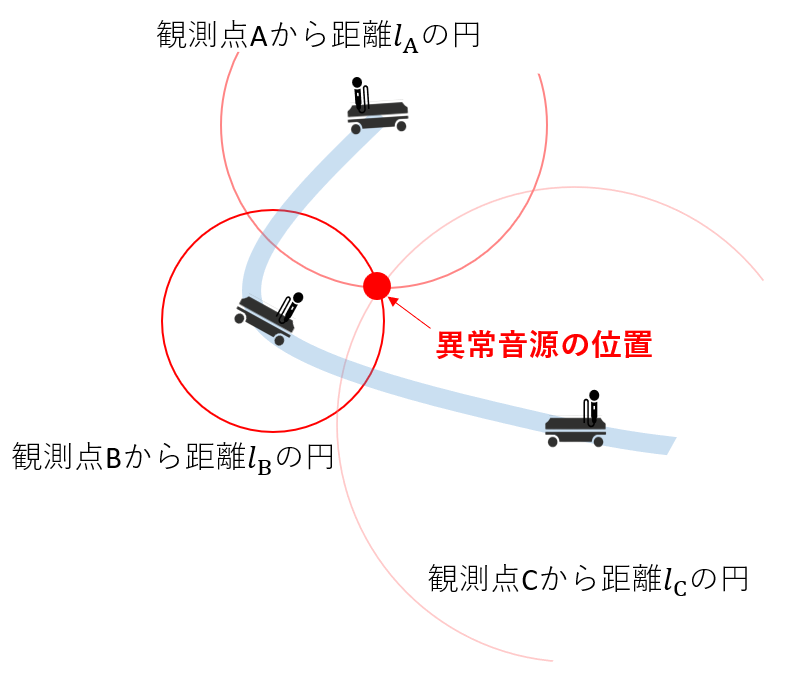
\includegraphics[keepaspectratio, width=0.8\linewidth]{chap3/localization.png}
    \caption{異常音源の位置推定の概念図}
    \label{fig:localization}
  \end{figure}

\subsection{最適化を用いた異常音の位置推定}

前節では異常音源の位置を三辺測量の考え方で説明したが,実環境ではノイズなどの影響により,各地点における異常音源までの距離推定 $d(\mathbf{p}_i,\mathbf{p}_a)$ に誤差が含まれる.
理想的には\refeq{eq:distance}が成り立つはずだが,実際には
\begin{equation}
    d(\mathbf{p}_i, \mathbf{p}_a) = \sqrt{\frac{\alpha}{E_i}} + \epsilon_i.
\end{equation}
となり,式中の右辺には観測や環境に起因する誤差 $\epsilon_i$ が含まれる.

このような誤差のために,理想的な意味での解(すべての地点で誤差がゼロとなる解)は存在しない.
そこで,本研究では経路上のすべての地点における異常音源までの距離の集合 $\{d(\mathbf{p}_i, \mathbf{p}_a)\}$ を利用し,$\epsilon_i$ が最小になるような\( \mathbf{p}_a \)を見つけることで,異常音源の位置推定を行う.

このような$\epsilon_i$の最小化には最小二乗法や重み付き最小二乗法などを用いることで解析的に解くことも考えられるが,本研究では多数の地点での観測データを活用することを前提としているため
,逆行列の計算が大規模になり実装や計算コストの面で困難になる.
そのため,数値的な最適化アルゴリズムを活用し,ノイズを含む実観測値に対しても適切に異常音源の位置を求める.

さらに,音は空間的に減衰するという性質上,異常音源から遠い地点でのエネルギー値は小さくなり,推定距離の精度が低下しやすい.
そのため,遠い地点の情報ほど推定値がノイズの影響を大きく受ける.
そこで,エネルギー値に応じた重みづけを損失関数の中で行うことで,異常音源から近い地点で計測された距離情報を重要視するような定式化を行う.
具体的な最適化の関数を以下に示す.

\begin{equation}
    \min_{\mathbf{p}_a} \sum_{i=1}^{N} w_i \left( \sqrt{\frac{\alpha}{E_i}} - d(\mathbf{p}_i, \mathbf{p}_a) \right)^2.
\end{equation}

\begin{equation}
    {w_i} = \sqrt{\frac{E_i}{\alpha}}.
\end{equation}

ここで,$w_i$ は重みを表し,$E_i$ は地点 $\mathbf{p}_i$ における正常音との差分エネルギー値,$d(\mathbf{p}_i, \mathbf{p}_a)$ は地点 $\mathbf{p}_i$ と異常音源 $\mathbf{p}_a$ との距離を示す.
この最適化問題を解くことで,異常音源の位置を推定することができる.

\end{document}
